\section{Network robustness}
The goal of studying network robustness is to see how a network behaves under some kind of failure. The most common form of failure that is studied is the removal of one node from a network. If the node is chosen at random, we call this a \emph{random failure} but if the node is chosen according to some heuristics, then we are talking about a \emph{targeted attack}. After the removal many properties of the network will change, but the one that concerns us the most is the probability $P_\infty$ with which a randomly selected node is part of the giant component.
In this section we will discuss some theoretical results and compare them with failure simulations on the Trainline network.

\subsection{Random failures}
When we gradually remove nodes from a network $P_\infty$ gets lower, up until it reaches zero. Under some condition, the network may undergo a phase transition and lead to $P_\infty$ reaching zero with a sharp drop, way before all of the nodes have been removed. This phase-transition behavior has been studied thoroughly within the framework offered by \emph{percolation theory} \cite{disorderedSystems}.
The results show that in a random network, the order parameter $P_\infty$ follows
\begin{equation*}
    P_\infty(f) \propto (f_c-f)^{\beta_f},
    \label{eq:percolation}
\end{equation*}
where $f$ is the fraction of nodes removed from the network, $f_c$ is a value dependent on the lattice type and $\beta_f$ is a \emph{critical exponent}. For reference, the value of $f_c$ for a two-dimensional square lattice is $f_c \approx .407$ and the value of $\beta_f$ is $\beta_f = 5/36$ (which is universal for lattices of dimension $2$).

When dealing with networks with an arbitrary degree distribution, however, we observe a different behavior. Relevant to us is the case of scale-free network, in which we do not see a sharp phase transition (for random failures, that is) but instead we find a steady, slow decline of $P_\infty$. Actually it can be proven that, for a network with an arbitrary degree distribution, we have a critical threshold $f_c$ on the fraction of nodes that we can remove, after which the network will completely lose its giant component. $f_c$ is given by \cite{barabasi16, molloyreed}:
\begin{equation}
    f_c = \ - \frac 1 {\frac {\langle k ^2 \rangle}{\langle k \rangle} - 1}.
    \label{eq:fc}
\end{equation}
Equation \eqref{eq:fc} predicts two different possible behaviors for scale-free network, depending on the value of $\gamma$:
\begin{itemize}
    \item For $\gamma < 3$, $\langle k^2 \rangle$ diverges and thus we get $f_c \to 1$ in the $N \to +\infty$ limit. This means that, in order to fragment the network, we need to remove all of its nodes.
    \item For $\gamma > 3$ we have that $f_c$ is independent of network size $N$, but depends only on $\gamma$ and $k_{\min}$. This behavior, proven in \cite{barabasi}, is the same as what we see in a random network: the network falls apart once a certain fraction of its nodes is removed.
\end{itemize}

I run a simulation on the Trainline network (\autoref{fig:random-failures}). Each data point in the plot is obtained by removing a certain fraction of nodes from the network and counting how many of the nodes are part of the giant component. This process is repeated $16$ times for each data point and the graph reports the standard deviation of all the results. The behavior we see is exactly what we expect from a scale free network with $\gamma < 3$. This result is great, as it indicates that the Trainline network is resilient to random failures of its node.
If, for example, a city were to be excluded from the network due to economical or environmental issues, the rest of the network would be able to keep working without any issues.

\begin{figure}[h]
    \centering
    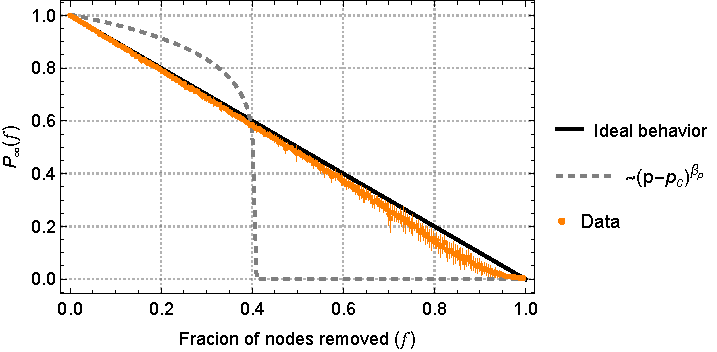
\includegraphics[width=1\linewidth]{report/assets/raindomFailuresPlot.pdf}
    \caption{Simulation of resilience of the network to random failures. Multiple runs were performed in which a certain number of nodes chosen at random was removed from the network. The graph shows the fraction of nodes that are still part of the giant component after the removal. The dashed, gray line is what we would expect to see if the network was wired like a 2-dimensional square lattice (null hypothesis).}
    \label{fig:random-failures}
\end{figure}


\subsection{Targeted attacks}
We have seen that scale free network are ideal if the mode of failure of the network is the removal of random nodes. What happens in the case of a targeted attack? 

\subsubsection{Attacking nodes}
We consider the case in which a potential attacker manages to disable the nodes in order of importance; that is, targeting the highest-degree node first. When this is the case, scale-free network do fail, and after only a small fraction of the nodes are removed \cite{barabasi12}.
It is possible to derive \cite{barabasi240} the following equation, whose solutions are the critical fraction of nodes that need to be removed by an attacker in order for the network to break apart completely:
\begin{equation}
    f_c^{\frac{2-\gamma }{1-\gamma }}= 2+ \frac{(2-\gamma )} {3-\gamma } k_{\min } \left(f_c^{\frac{3-\gamma }{1-\gamma }}-1\right).
    \label{eq:fc-attack}
\end{equation}
In our case, using the values of $k_{\min}$ and $\gamma$ that we obtained above, we get that $f_c = .235$ is the only acceptable solution. 

Again, we can confirm this behavior by running a simulation in which we remove the highest degree nodes, one at a time, and compute $P_\infty$ at each step.
The result (\autoref{fig:node-attack}) shows a fast, steady decline up to $f=.2$, after which we have a steep drop. At $f=.3$, more than $95\%$ of the network is now unreachable. This behavior matches what the theory predicts and highlights one very big weakness of the Trainline network.

\begin{figure}[h]
    \centering
    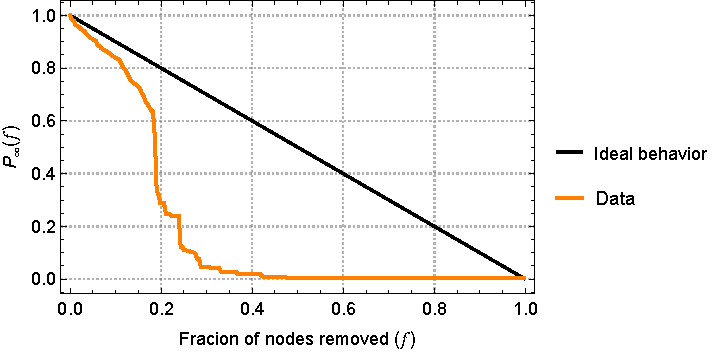
\includegraphics[width=1\linewidth]{report/assets/nodeAttackPlot.pdf}
    \caption{Simulation of resilience of the network to targeted attacks. One simulation was performed in which the highest-degree nodes were removed sequentially. The graph shows the fraction of nodes that are still part of the giant component after the removal.}
    \label{fig:node-attack}
\end{figure}

\subsubsection{Surviving communities}
We can make one interesting observation by plotting the community structure of the network just after the big drop at $f=.2$ (\autoref{fig:survivor-communities}). From this we can see that, even if the network is now fragmented, the individual communities more or less managed to survive. A network in this state would still be able to carry out some of its work; this means that the current attack strategy is a little less effective than what the calculations predict.

\begin{figure}[h]
    \centering
    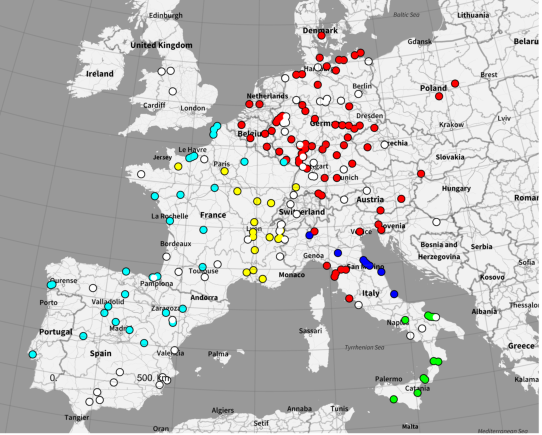
\includegraphics[width=1\linewidth]{report/assets/survivorCommunitiesVertexPlot.pdf}
    \caption{Survivor communities after the removal of the top $50$ highest-degree nodes. We can see that the community detection algorithm still manages to pick up some communities, meaning that some areas of the network manage to stay locally connected. The white dots group all the nodes that do not belong to any of the biggest communities.}
    \label{fig:survivor-communities}
\end{figure}


\begin{figure}[h!]
    \centering
    \begin{subfigure}[h]{\linewidth}
        \centering  
        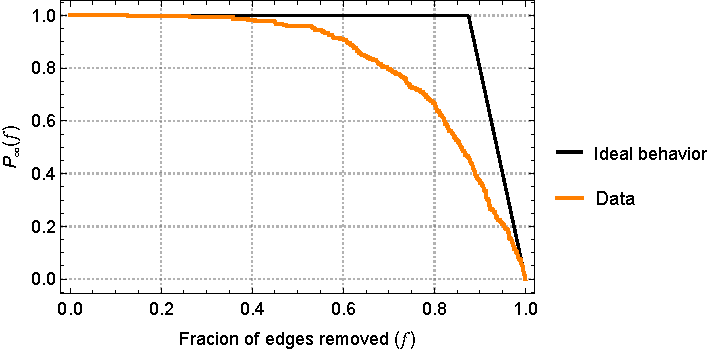
\includegraphics[width=\linewidth]{report/assets/edgeAttackGraph.pdf}
        \caption{Results of removing highest-througphut edges.}
        \label{fig:edge-attack-graph}
    \end{subfigure}
    \hfill
    \begin{subfigure}[h]{\linewidth}
        \centering
        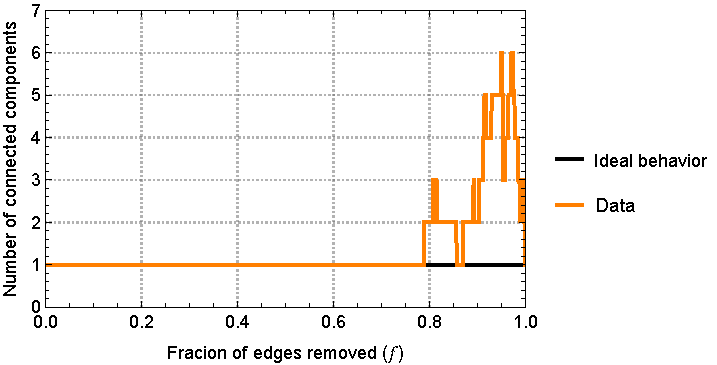
\includegraphics[width=.95\linewidth]{report/assets/edgeAttackComponentsPlot.pdf}
        \caption{Number of connected components after the highest-throughput edges are removed. The value of $1$ indicates that the whole network stays connected, up until the top $80\%$ of the edges are removed.}
        \label{fig:edge-attack-components}
    \end{subfigure}
    \caption{Simulation of resilience of the network to targeted edge attacks. One simulation was performed in which the highest-throughput edges were removed sequentially. The graph (a) shows the fraction of nodes that are still part of the giant component after the removal, while the graph (b) shows the number of components in which the network is split after the removal.}
    \label{fig:edge-attack}
\end{figure}


\subsubsection{Attacking edges}
To conclude this section I also wanted to explore how the network would behave if an attack were to be performed on the links, instead of on the nodes.
The rationale behind this is that train tracks, contrary to train stations, cannot be monitored throughout their whole length and thus could be more easily targeted by a destructive attack\footnotemark.

There is some research \cite{edgeremoval} on what is the best edge attack strategy, but it is mostly based on empirical results and lacks a deep theoretical study.
For my simulation, I chose the simplest attack strategy possible: remove the links according to their magnitude in the rate matrix $W$, starting from the highest to the lowest. The results (\autoref{fig:edge-attack}) show that the network is mostly untouched by this kind of attack. As a matter of fact, if we confront the two graphs in \autoref{fig:edge-attack-graph} and \autoref{fig:edge-attack-components} we can see that, even though $P_\infty$ starts to decay after $f=.4$, the number of connected components of the network stays constant throughout, up until $f=.8$.
This means that the removal of edges would, at most, only leave out singular nodes without fragmenting the network.

Given that edge attacks would be easier to execute, this result shows that the Trainline network might be more robust than what could transpire from the data in the previous section.



\footnotetext{Again, I would like to stress out that the Trainline network is very different from the European train track network. Nonetheless, in order for a link to exist on the Trainline network, there need to exist a physical track link as well.}


\subsection{Summary of the results}
Equations \eqref{eq:fc} and \eqref{eq:fc-attack} can be plotted together to show the predicted breakdown threshold of a scale-free network under the two possible moedes of failure. The result (\autoref{fig:fc-plot}) shows that for low values of $\gamma$, scale-free networks are susceptible to targeted attack and resilient to random failures. If the value of $\gamma$ gets too high, the value of $f_c$ tends to converge for both cases.

\begin{figure}[h]
    \centering
    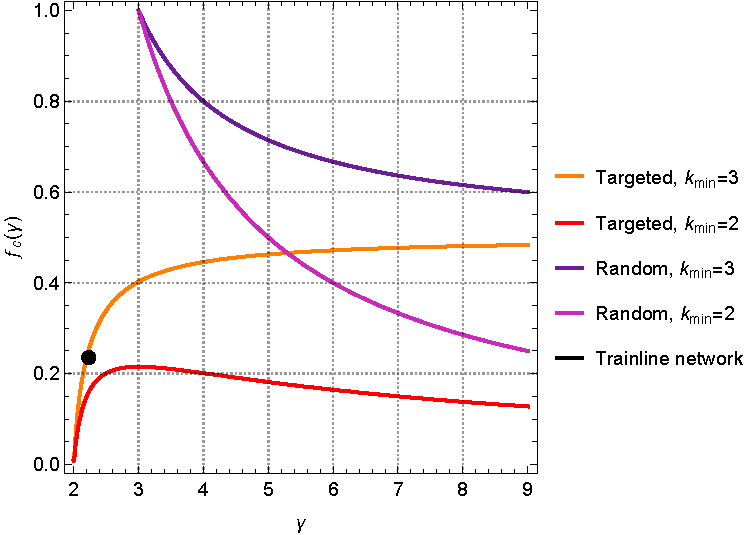
\includegraphics[width=1\linewidth]{report/assets/fcPlot.pdf}
    \caption{Plot of equations \eqref{eq:fc} and \eqref{eq:fc-attack}, which summarizes the resilience of a network as a function of the parameters $\gamma$ and $k_{\min}$. We can see that for low values of $\gamma$ a scale-free network is resilient to random failures but vulnerable to attacks. Over a certain threshold, the values fo $f_c$ tend to converge for both types of failures.}
    \label{fig:fc-plot}
\end{figure}